\documentclass{article}
\DeclareMathSizes{10}{10}{7}{7}
\usepackage{amsmath}
\usepackage{ amssymb }
\usepackage{tikz, graphicx}
\usepackage{geometry}
\usepackage[makeroom]{cancel}
\usepackage[export]{adjustbox}
\DeclareMathOperator{\sech}{sech}
\usepackage{subfig}
% http://www.mathworks.com/matlabcentral/fileexchange/8015-m-code-latex-package
\usepackage[framed,numbered,autolinebreaks,useliterate]{mcode}
\usepackage{hyperref}
\hypersetup{
    colorlinks=true,
    linkcolor=blue,
    filecolor=magenta,      
    urlcolor=blue,
    }
\usepackage{float}
\restylefloat{table}

\geometry{legalpaper, margin=0.7in}

\title{3AN Project 2\\ What happened when two waves crossed the road}
\author{Liam Watson WTSLIA001}
\begin{document}
\maketitle
\section{Introduction and physics}
We wish to better understand the interaction between colliding solitons within some optical communication media such as firbre obtic cable used for audio or network communications. 
We can model optical pulses in a media with saturation nonlinearity properties using the following modified nonlinear  Schr¨odinger equation:
\begin{align}
i\psi_t + \psi_{xx} + \frac{2|\psi|^2\psi}{1+S\sin(|\psi|^2)} = 0
\end{align}
Note that we impose periodic boundary conditions to the Schr¨odinger equation. \\
We can study the collisions of N solitons by choosing our initial configuration as the sum of N solitons separated by a sufficiently large distance as follows:
\begin{align}
\psi (x,0) = \sum_{j=1}^N A_j \sech(A_j (x-x_j))e^{iv_j(x-x_j)}
\end{align}
In the following sections we will study the soliton collisoons for different values of the nonlinearity saturation $S\in(-1,1)$, the velocity $v$ the intersoliton distance $|x_k-x_j|$. \\
This analysis will be done using two different numerical methods, namely the split-step and finite difference methods. To ensure that any insight gained from either method is consistent we will ensure that the following conserved quantity remains within a maximum deviation of $\varepsilon = 10^-5$.
\begin{align}
N = \int_{-\infty}^\infty |\psi|^2 dx
\end{align}
Additionally we will compare the execution time of both numberical methods for the given $\varepsilon$
\section{Derivation of needed numerical method formula}
In the following two sections we will discuss the derivation of the formula needed for the implementation of the two numerical methods. 
\subsection{Split-Step}
The Split-step method relies on splitting the differential equation (1) into a nonlinear part using it to solve the linear part. After some intermediate steps we find that the nonlinear part can be expressed as
\begin{align}
\psi = \psi(x,0) e^{\frac{2iCt}{1+S\sin(c)}}, C = |\psi|^2
\end{align}
Note that we know $C$ is constant as 
\begin{align}
\psi_t \psi bar + \psi_t bar + \psi = 0 \implies \frac{\partial}{\partial t}(\psi\psi bar) = 0 \implies |\psi|^2 = C
\end{align}
We move onto the linear part which after using a fuourier sieries expansion over our discretized region can be expressed by
\begin{align}
W(x,t_{k+1}) = \sum_{-N/2}^{N/2-1} W_k e^{\frac{2 \pi i k x}{L}}
\end{align}
\subsection{Finite Difference}
There are three main methods that we can use for a finite difference expansion namely, Explicit, Implicit and Crank Nicolson. \\
Crank Nicolson method produces the following expression for (1) after discretizing in time and space. 
\begin{align}
i\psi_{i,k+1} + \frac{\tau}{2h^2}(\psi_{j-1,k+1} -2\psi_{j,k+1} + \psi_{j+1,k+1}) = i\psi_{j,k} - \frac{\tau}{2h^2}(\psi_{j-1,k}-2\psi_{j,k} + \psi_{j+1,k}) - \frac{2\tau |\psi|^2 \psi}{1+S\sin|\psi|^2}
\end{align}
\section{Implementation}
IMPL
\section{Split-Step}
\begin{lstlisting}
clear all; %Ensure testing is not effected by past computation
clc;
tiledlayout(2,2)
figCount = 0;

for v = [0.5, 1, 2 , 10]
    figCount = figCount + 1;
L = 100; %Simulation space interval
N = 1000; %Number of mesh points
h = L/N; %Size of mesh spacing
x = 0:h:(L-h); %Discretized spacial interval
tau = h^2/3;%The method is explicit so there is a stability condition
A1 = 1; %Aplitude of soliton 1
A2 = 1; %Aplitude of soliton 2
S = 0.9; %Saturation of nonlinearity
xPos1 = 30;  %Starting position of wave peak in x direction
xPos2 = 60; %Starting position of wave peak in x direction
v1 = v;
v2 = -v;
%v1 = 1;  %Velocity of soliton 1
%v2 = -1; %Velocity of soliton 1
psi = A1*sech(A1*(x-xPos1)).*exp(1i*v1*(x-xPos1))...%Soliton 1 Inital
      + A2*sech(A2*(x-xPos2)).*exp(1i*v2*(x-xPos2));%Soliton 2 Inital
%plot(x,abs(psi))%Plot inital configuration. Removed for testing speed
time=3000/v; %Max time

%Used for 3D plot
X = [x];
Y = [abs(psi)];
Z = [0:time];
%%%%%%%%%%%%%%%%
vec2 = 4*pi^2/L^2*[0:N/2 - 1 -N/2:-1].^2;
for ti=1:time
    psi = psi.*exp((tau*2.i*abs(psi).^2)./(1+S*sin(abs(psi).^2))); %Update psi
    psi = ifft(fft(psi).*exp(-1i*tau*vec2)); %Update psi with FFT and IFFT approxmiation
    Const = trapz(x,abs(psi).^2); %The conserved quantity
    %X = [X;x];
    Y = [Y;abs(psi)]; %Used for 3D plot
    
    %plot(x,abs(psi)), drawnow %Plot 2D updated solution for time t
end
%nexttitle
subplot(2,2,figCount);
h = surf(X,Z,Y) %Plot 3D, x, t, psi
set(h,'LineStyle','none')
%Const = round(Const,6,'significant');
title("|v|=" + v + ",   D=" + compose("%9.7f",Const))
end
\end{lstlisting}
\pagebreak
\subsection{Finite Difference}
\begin{lstlisting}
clear all; %Ensure testing is not effected by past computation
clc;
tiledlayout(2,2)
figCount = 0;

for v = [0.5, 1, 2 , 10]
    figCount = figCount + 1;
L = 100; %Overall simulation interval
N = 3000; %Number of space subdivisions
h = L/N; %Size of mesh spacing
x = [0:h:(L-h)]'; %Space mesh
tau = h^2/3; %Time step

A1 = 1; %Inital amplitude of soliton 1
A2 = 1; %Intial amplitude of soliton 2
S = 0.0; %Nonlinarity saturation
xPos1 = 30; %Starting position of wave peak in x direction
xPos2 = 60; %Starting position of wave peak in x direction
v1 = v;
v2 = -v;
%v1 = 1; %Velocity of soliton 1
%v2 = -1; %%Velocity of soliton 2
psi = A1*sech(A1*(x-xPos1)).*exp(1i*v1*(x-xPos1))...%Soliton 1 Inital
      + A2*sech(A2*(x-xPos2)).*exp(1i*v2*(x-xPos2));%Soliton 2 Inital

%plot(x,abs(psi)) %Plot inital configuration. Removed for testing speed

s = tau/h^2; %code simplifcation
s2 = s/2; %code simplifcation

A = diag((1i-s)*ones(N,1),0)... %Set the FD matrix values on diagonals
    +diag(s2*ones(N-1,1),1)...
    +diag(s2*ones(N-1,1),-1);
A(1,N) = s2; %Set periodic BC elements in matrix A
A(N,1) = s2;
A = inv(A);
rhs = zeros(size(x)); %Create RHS vector
time = 3500/v; %Max time

X = [x]; %Used for 3D plot
Y = [abs(psi)];%Used for 3D plot
Z = [0:time];%Used for 3D plot
for t=1:time %Loop until max time reached   
    rhs(2:N-1) = (1i + s)*psi(2:N-1)-s2*psi(1:N-2)... %Update RHS
        - s2*psi(3:N)...
        - (2*tau*(abs(psi(2:N-1)).^2).*psi(2:N-1))./(1+S*sin(abs(psi(2:N-1)).^2));
        %- (tau*(abs(psi(1:N-2)).^2).*psi(1:N-2))./(1+S*sin(abs(psi(1:N-2))))...
        %- (tau*(abs(psi(3:N)).^2).*psi(3:N))./(1+S*sin(abs(psi(3:N))));
        
    
    rhs(1) = (1i + s)*psi(1) -s2*psi(2) -s2*psi(N)...
        -(2*tau*abs(psi(N)).^2.*psi(N))/(1+S*sin(abs(psi(N)).^2));
        %-(tau*abs(psi(N)).^2.*psi(N))/(1+S*sin(abs(psi(N))))...
        %-(tau*abs(psi(2)).^2.*psi(2))/(1+S*sin(abs(psi(2))));
        
    
    rhs(N) = (1i + s)*psi(N) -s2*psi(1) -s2*psi(N-1)...
            -(2*tau*abs(psi(N)).^2.*psi(N))/(1+S*sin(abs(psi(N)).^2));
            %-(tau*abs(psi(N-1)).^2.*psi(N-1))/(1+S*sin(abs(psi(N-1))))...
            %-(tau*abs(psi(1)).^2.*psi(1))/(1+S*sin(abs(psi(1))));
    %psi = A\rhs;
    psi= A*rhs; %Solve for psi
    Y = [abs(psi) Y]; %%Used for 3D plot
    Const = trapz(x,abs(psi).^2); %The conserved quantity
    
    %plot(x,abs(psi)), drawnow %Plot 2D updated solution for time t
end
subplot(2,2,figCount);
h = surf(X,Z,Y') %Plot 3D, x, t, psi
set(h,'LineStyle','none')
title("|v|=" + v + ",   D=" + compose("%9.7f",Const))
end
\end{lstlisting}
\pagebreak
\section{Results and Discussion}
\subsection{Performance and accuracy}
We choose $S=0$, $v1 = 1$, $v2 = -1$, $x_1 = 30$, 
In order to test both methods performance we must calibrate the two methods hyperparameters so that the conserved qunatity deviation $\varepsilon < 10^{-4}$. We find after some initial testing that the Finite Difference method deviates more than the Split Step method for any given mesh spacing. This is likely due to the nonlinear Shroedinger equation not being integrable. The Split Step method avoids this as both the linear and nonlinear parts are integrable where as the Finite Difference method attempts to directly solve the equation (1). \\
Calibration results in the following choices of parameters for testing. 
Finite Difference: $N=2000$ and $\tau = h^2/3 = 8.333x10^{-4}$ \\
Since $\tau$ is linked to the choice of $N$ we must choose the same $\tau$ for the Split Step method. The resulting conserved constant near the collision is $4.000089807509760$. \\
Split Step: $N=150$ and $\tau = 8.333x10^{-4}$. The resulting conserved constant is approxmimately $4.000088112839693$\\
The testing was completed using Matlabs tic toc routine whith timing starting before any variable assignment and after $6000$ time steps. 
We ensure consistency by removing all plotting routines and their required variables, printing routines. Additionally, we clear all cached data.
Run time analysis:\\
Split Step: Elapsed time is 0.256348 seconds.\\
Finite Difference:  Elapsed time is 3416.665484 seconds. This is a very poor result which can be improved with some optimization of memory by declaring vectors before hand using the zeros routine and calculating the inverse of our $A$ matrix once before the loop rather than every itteration. Which results in Elapsed time is 51.400328 seconds.


\subsection{Analysis of numerical solutions}
\begin{enumerate}
\item

This papers' scope is too small to examine the effects of varing the saturation of nonlinearity, velocity and intersoliton distances for both numerical schemes. First let us verify that both schemes produce similar results.

\begin{figure}[htp]

\title{Finite difference method solution to equation (1)\\}
\centering
\includegraphics[scale=0.3]{Capture.PNG}
\caption{\\The above figure is the solution of equation (1) using the Finite Difference method over 6000 time steps, $N = 2000$, $v_1=-v_2= 1$, $x_1=30$, $x_2=60$ and $S=0.5$. We can verify that this is the same result, qualitatively, that is produced by the split step method as seen in figure 2 bellow. }
\end{figure}


\begin{figure}[htp]
\title{Split Step method solution to equation (1)\\}
\centering
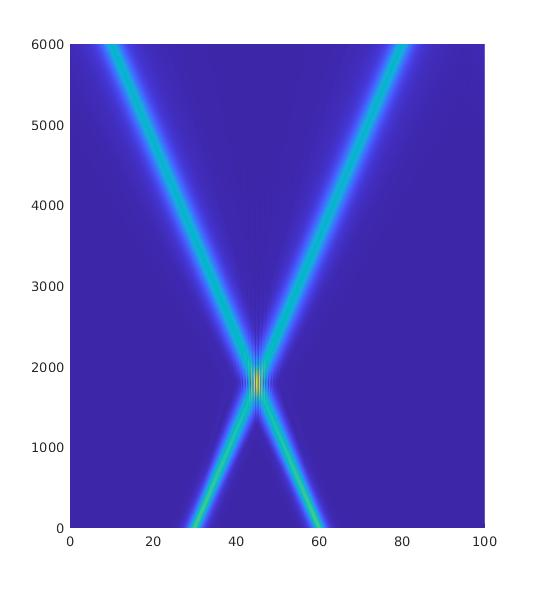
\includegraphics[scale=0.4]{Capture3.jpg}
\caption{As we can see the qualatative properties of the solutions are the same with split step being more computationally efficient and accurate as the conserved quantity vary more than $\varepsilon=10^{-12}$ with an $N=2000$ which is what will be used for the analysis of the different properties of the solitons.}
\end{figure}
\begin{figure}[htp]
\title{Figure 1 from a different perpective.\\}
\centering
\includegraphics[scale=0.32]{Capture2.PNG}
\caption{\\Here we can see that the qualitative properties of the solitons are best captured by a heat map. However, it is included to better demonstrate the amplitude of the solitons as well as the "interferance patterns" caused by the nonlinearity.}
\end{figure}
\item Testing small and large velocity \\
To keep testing consistent the following figures were obtained with $N=1000$ due to memory and processor restrictions. The maximum time was allowed to vary as was needed for the various velocities. 
\begin{figure}[htp]
\title{Solition heat maps for various velocities for $S=0$\\}
\centering
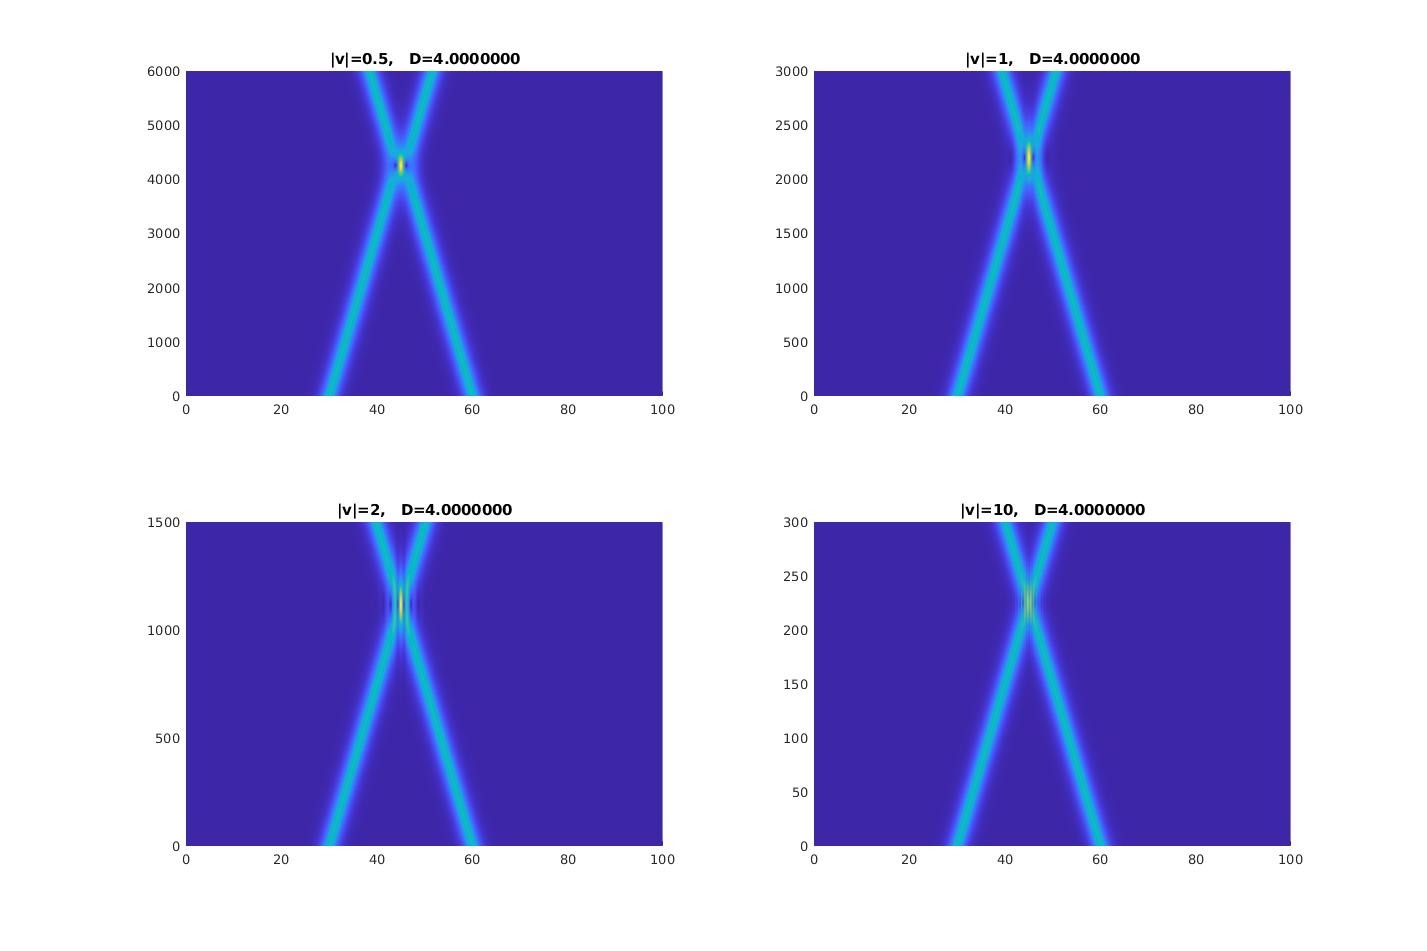
\includegraphics[scale=0.35,center]{3D_V_S0.jpg}
\caption{We can see that for small velocities 0.5 and 1 there is no unexpected behavior, the waves collide (adding amplitudes) and seperate without any secondary effects. As the velocity increases we start to see many large amplitude spikes that then seperate wihout any secondary effects. Additionally, the collision is elastic with the solitions having a constant amplitude before and after the collision.}
\end{figure}
\pagebreak
\begin{figure}[htp]
\title{A different angle for figure 4\\}
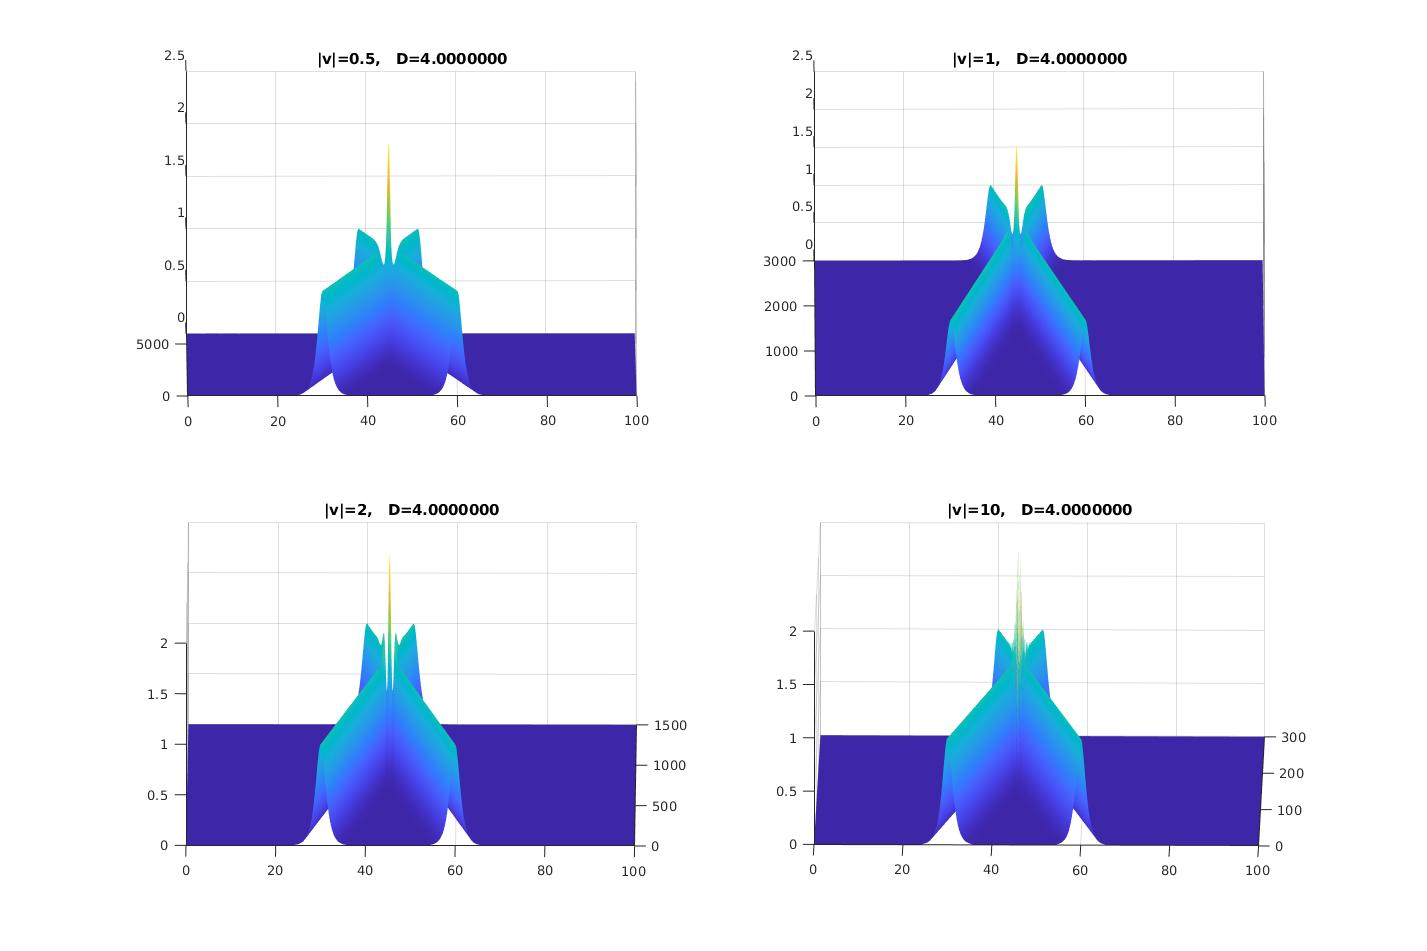
\includegraphics[scale=0.3,center]{3D2_V_S0.jpg}
\caption{We include this figure to demonstrate more clearly the "spikes" at the collision of the two solitons for large velocities}
\end{figure}

The result with zero nonlinearity is uninteresting with expected results appart from the spikes forming at the intersection of the two solitons. Let us now investigate positive nonlineariy $S$. 
\begin{figure}[htp]
\title{Solition heat maps for various velocities for $S=0.5$\\}
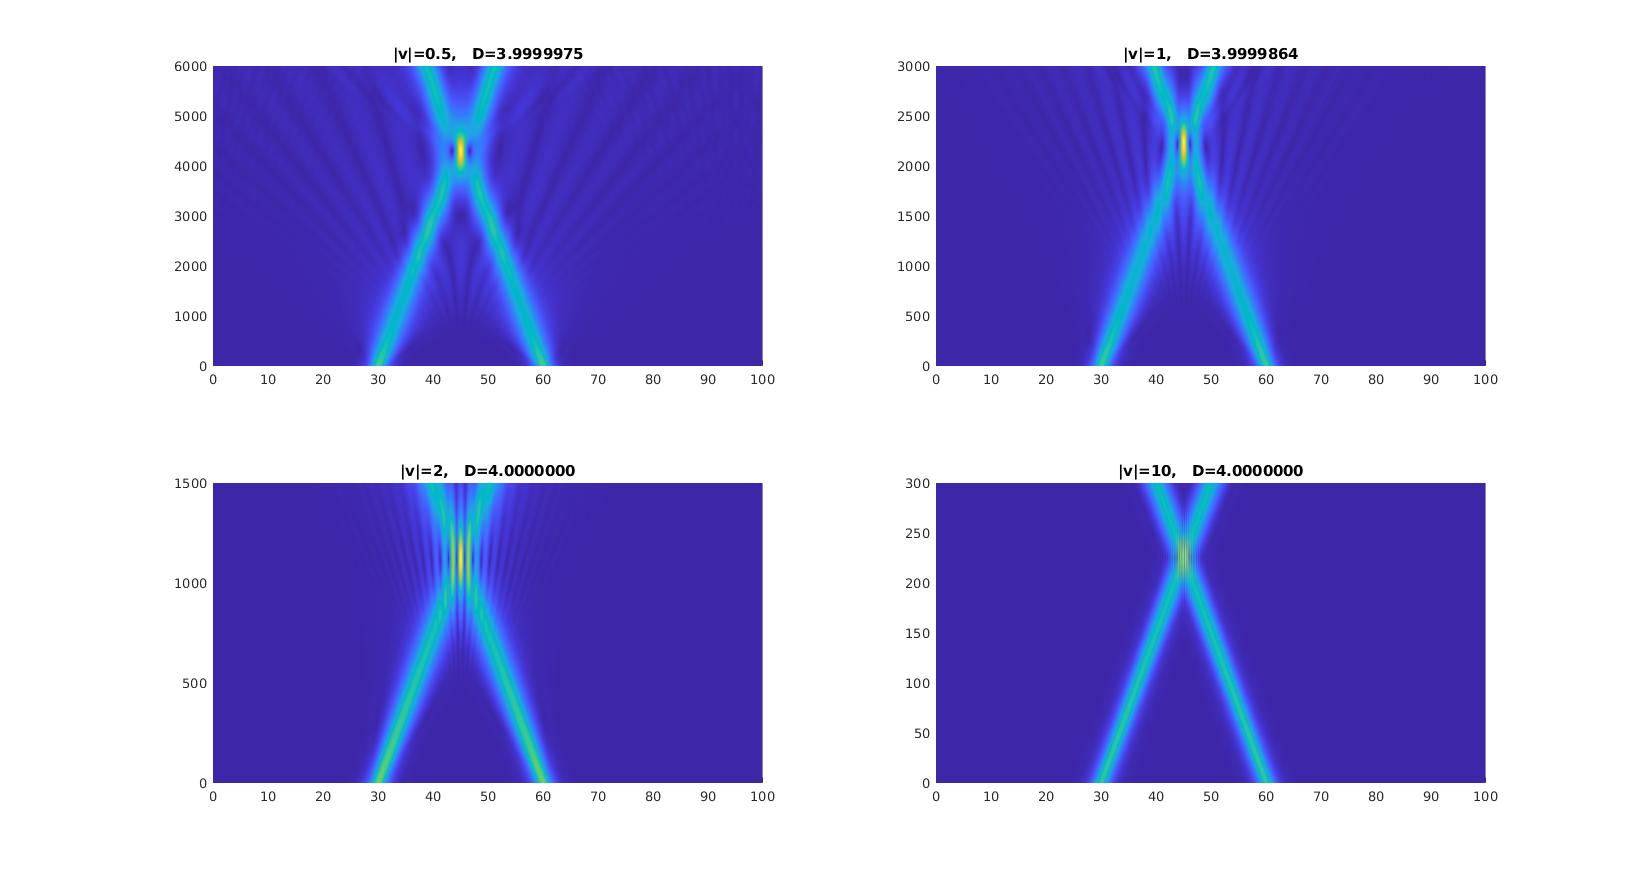
\includegraphics[scale=0.35,center]{3D_V_S05.jpg}
\caption{We can see that waves of smaller amplitude are produced for small velocities which decrease as we increase velocity.}
\end{figure}
\begin{figure}[htp]
\title{Solition heat maps for various velocities for $S=0.9$\\}
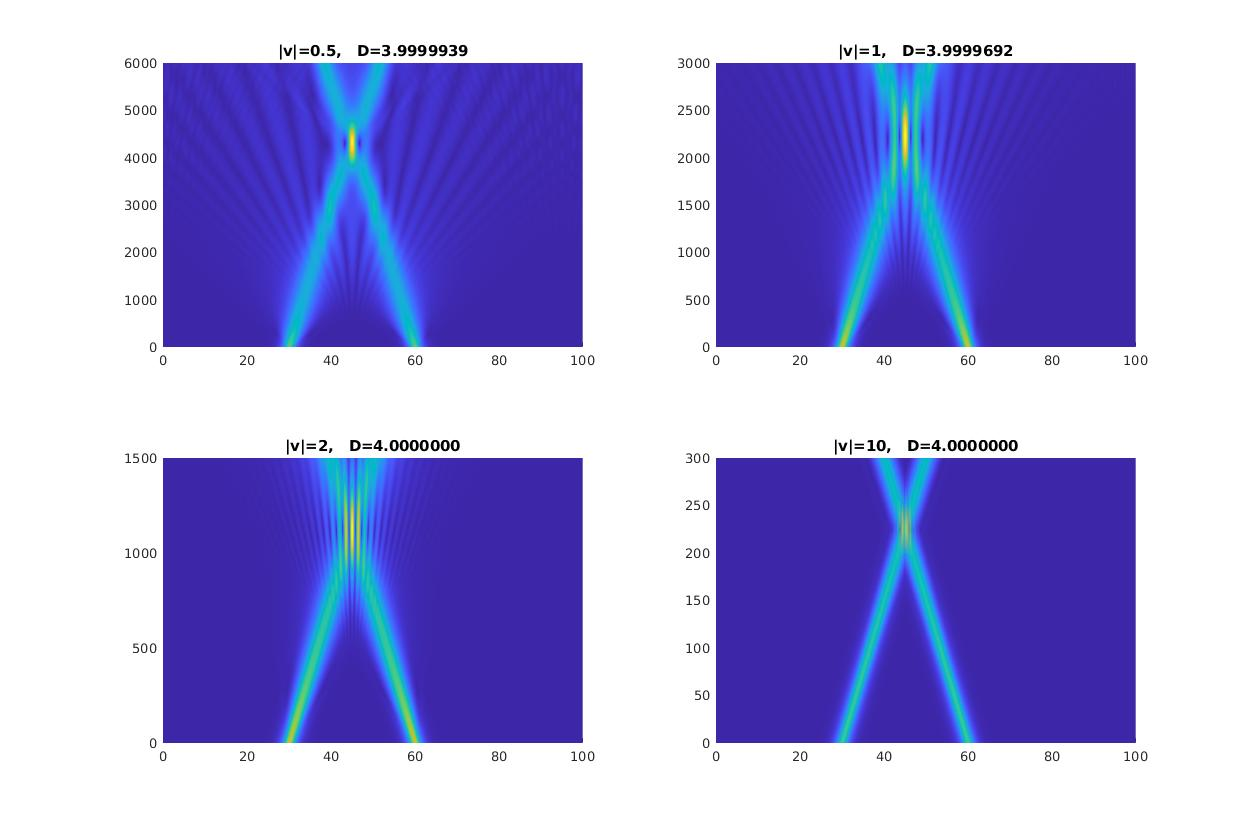
\includegraphics[scale=0.5,center]{3D_V_S09.jpg}
\caption{In the above figure we can see the same effect as in Figure 6, however, more pronounced}
\end{figure}
In figures 6 and 7 we can see unexpected formation of secondary waves that form before the collision of the two solitons and spread away from the intersection point. These secondary waves remove energy from the two initial solitions thus decreasing signal strength within the transmission medium. Aditionally, these smaller waves may be interpreted as an intentional to any reviever and thus we must be cautious of the sensitivity of the reciever two solition signals collide. \\
\item Negative nonlinearity \\
We know from before that phenominon incurred by some value of nonlinearity emphsized but not qunatatively changed for values of one sign (this was verified but not included in this paper for berevity) so we will only test $S = -0.9$.

\begin{figure}[htp]
\title{Solition heat maps for various velocities for $S=-0.9$\\}
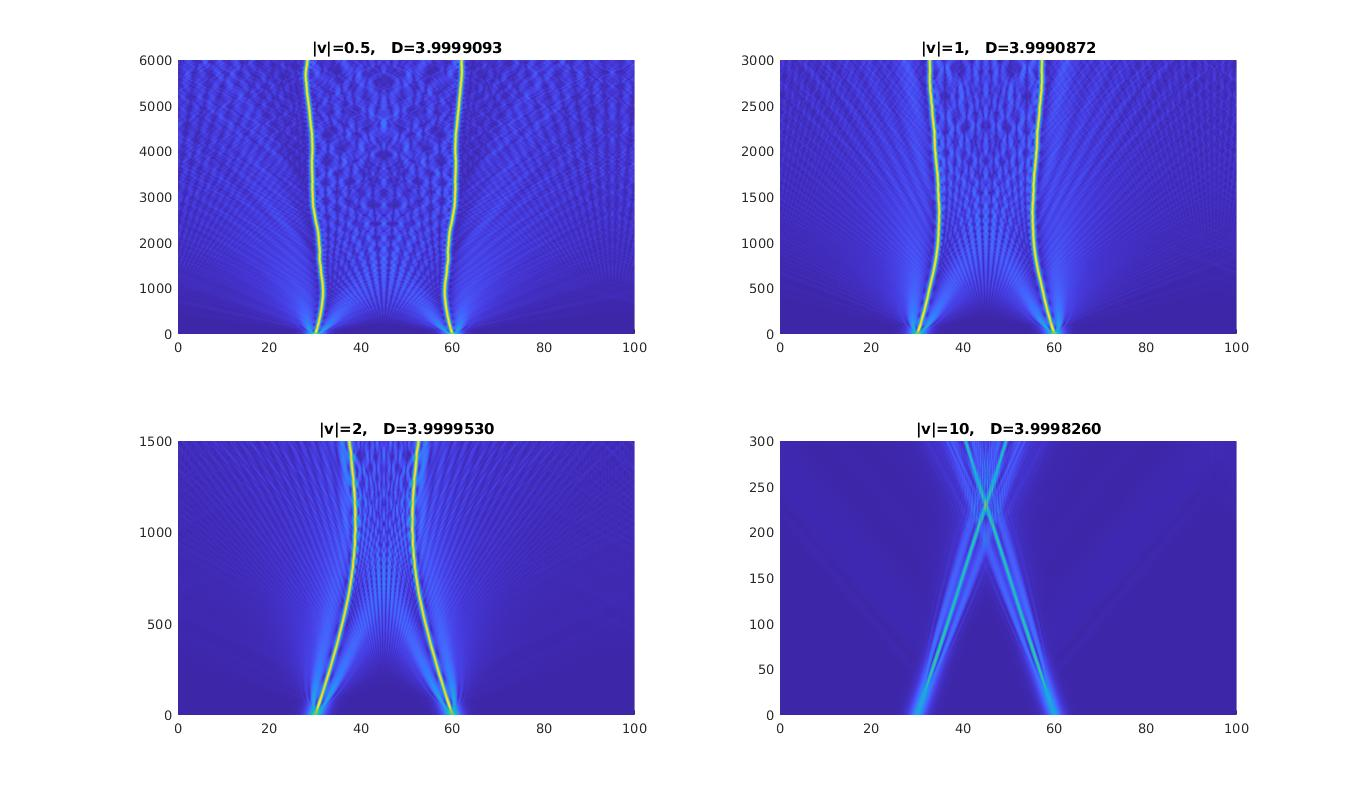
\includegraphics[scale=0.5,center]{3D_V_Sneg09.jpg}
\caption{Above we see some very interesting interactions that once again are reduced by higher velocity}
\end{figure}
In figure 8 we can see that for negative $S$ many small waves form within the medium that interact with each other giving a very distinct pattern. One can also note that for small velocities the solitions do not directly colide but rather seem to deflect with interactions and energy transfered via the smaller interferance waves. This effect would be detramental in information transer if velocities are small as the initial solitons seem to oscilate and lose velocity, however, information transfer is done using light which has a very high velocity of $2x10^{8} m/s$ which should reduce these effects dramatically. \\
\item Intersoliton distance \\ 
\begin{figure}[htp]
\title{Varying intersolution distance with $S=0$ and $S=0.5$\\}
\subfloat[$S=0$]{
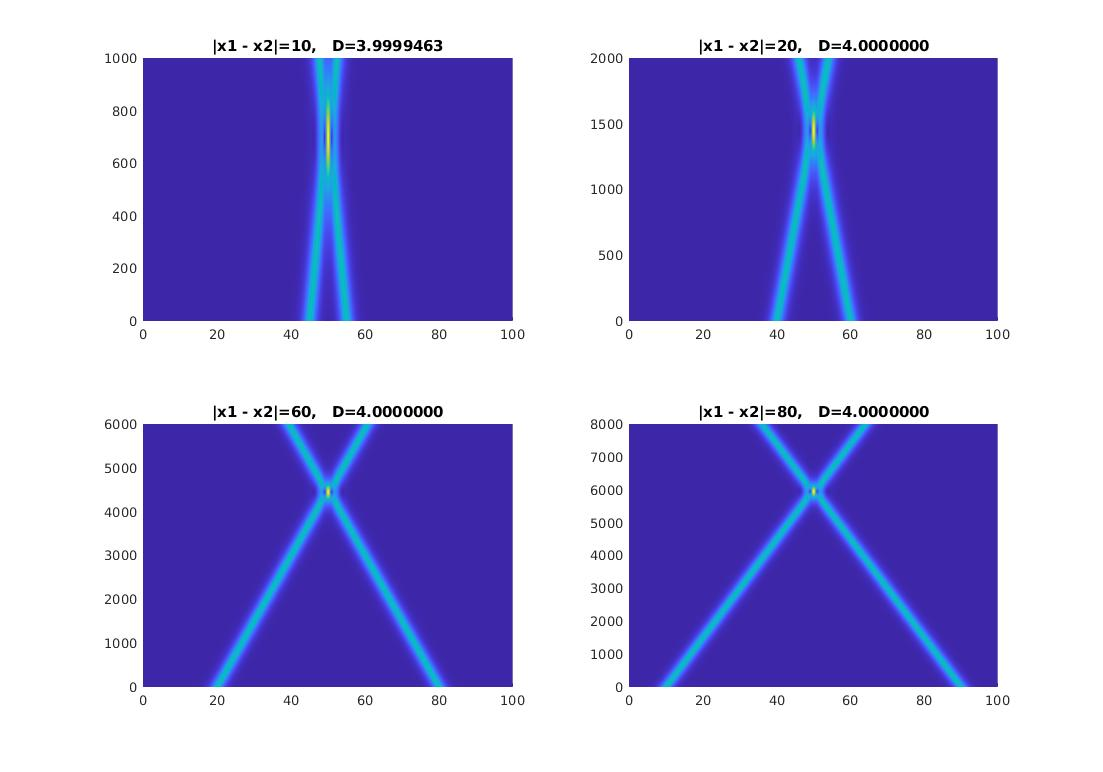
\includegraphics[scale=0.22]{3D_X_S0.jpg}}
\hfill
\subfloat[$S=0.5$]{
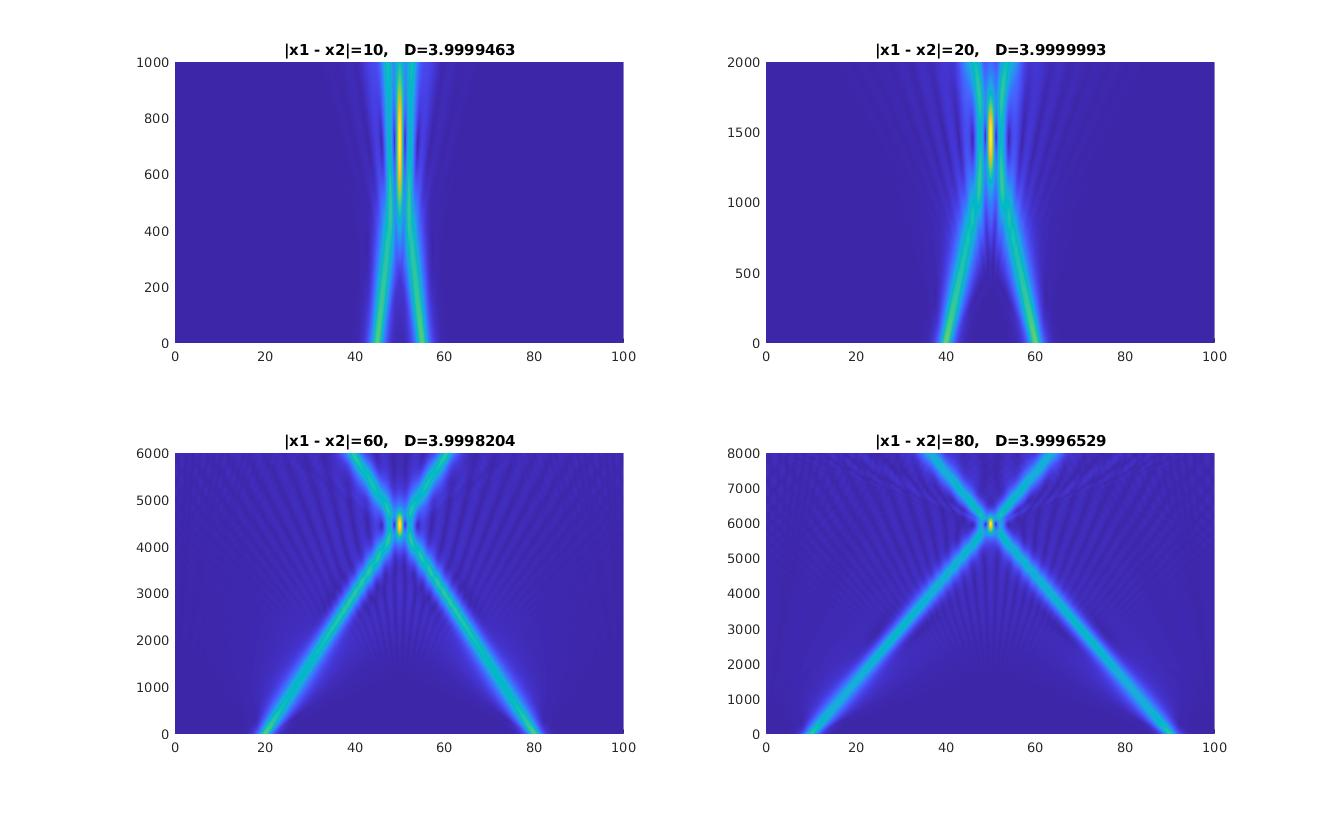
\includegraphics[scale=0.20]{3D_X_S05.jpg}}
\caption{Collision of 2 solions with $v_1=1$ and $v_2=-1$}
\end{figure}
Figures 9a and 9b show us that intersoliton ditance has little effect on the qualitative properties of the collision as 9a shows there is no effect on the simulation (note that the "steached" effect is due to the different time scales as closer solitions collide in short time). \\
\begin{figure}
\title{Varying intersoliton distance with $S=-0.5$\\}
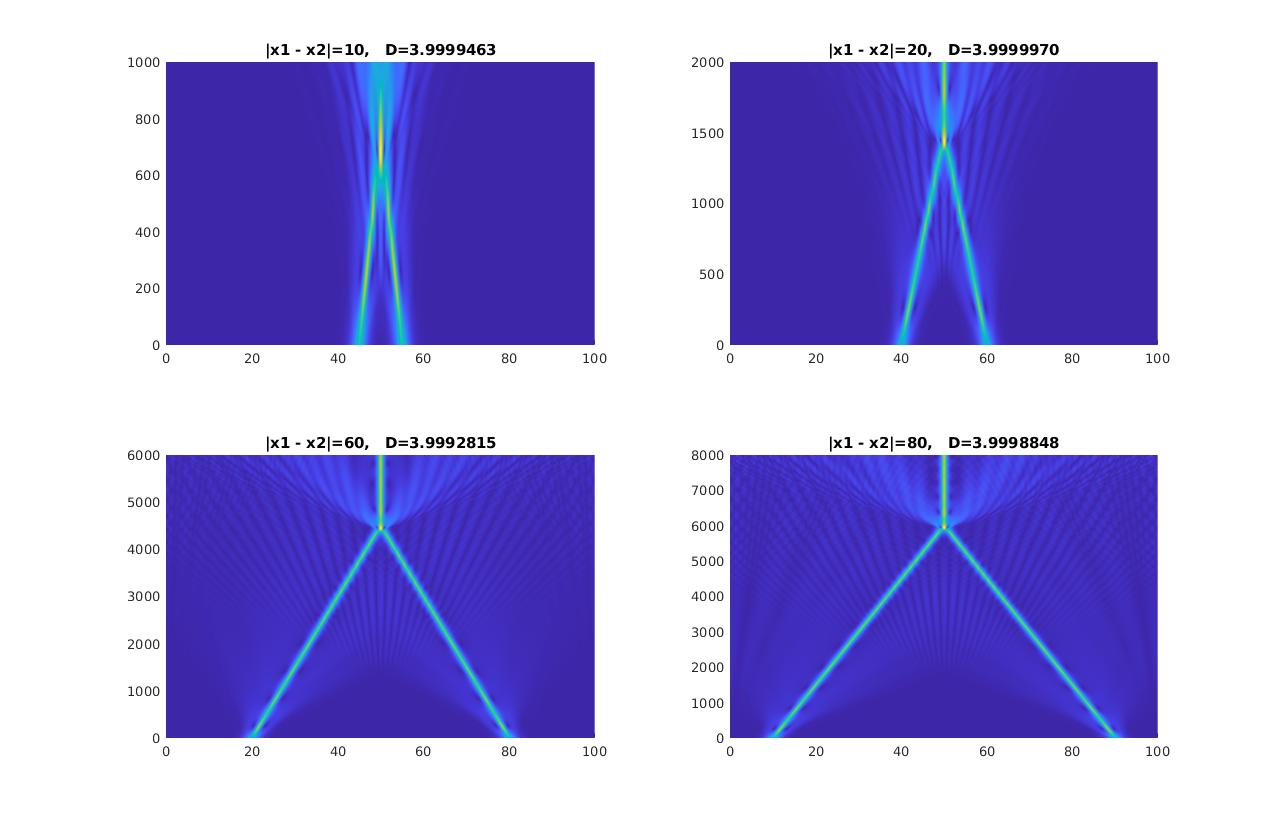
\includegraphics[scale=0.4]{3D_X_Sneg05.jpg}
\caption{Demonstrating standing wave and secondary waves}
\end{figure}
Figure 9 shows us that waves that are sufficiently far appart with negative nonlinear saturation form a standing wave surrounded by interferance. This phenomenon would be detramental for infomation transfer as only the secondary interferance waves would be transferred in the medium, however, this can be avoided with high enough velocity which is the case for optical waves. 
\end{enumerate}
\pagebreak
\section{Conclusion}
The numerical analysis of coliding solitons within this paper have indicated several phenomina (Standing waves, secondary waves, spikes and nonelastic collisions). These phenomenon are cuased by nonzero values for the nonlinear saturation $S$ which is typical for colliding solitions within optical media. However we discovered that the phenomenon in all cases are reduced in not entirely mitigated by high velocity initial solitions which is the case in optical transmission. The interferance (secondary waves) are somewhat of an issue as high velocity waves still produce these artifacts but one can easily mitigate them by calibrating the receivers sensitivity to ignore them, note that there is a chance that superposition of these smaller waves may result in their detection which will need to be corrected in software. \\
The collisions for zero nonlinear saturation were completely elastic with no energy being lost hoever this was not the case for nonzero values of $S$, this has implications for signal attenuation (signal loss over distance) which may need to be corrected for by some kind of relay to amplify the signal amplitude. \\
Recommandations for further analysis: One should use a numerical method that circumvents the nonintegrability of the Nonlinear shroeginer equation (1) such as split step to avoid numerical errors effecting results as well as for performance reasons. 

\end{document}